\documentclass[17pt]{beamer} %Makes presentation
%\documentclass[handout, 17pt]{beamer} %Makes Handouts
\documentclass[14pt]{beamer} %Makes presentation
%\documentclass[handout]{beamer} %Makes Handouts
\usetheme{Singapore} %Gray with fade at top
\useoutertheme[subsection=false]{miniframes} %Supppress subsection in header
\useinnertheme{rectangles} %Itemize/Enumerate boxes
\usecolortheme{seagull} %Color theme
\usecolortheme{rose} %Inner color theme

\definecolor{light-gray}{gray}{0.75}
\definecolor{dark-gray}{gray}{0.55}
\setbeamercolor{item}{fg=light-gray}
\setbeamercolor{enumerate item}{fg=dark-gray}

\setbeamertemplate{navigation symbols}{}
%\setbeamertemplate{mini frames}[default]
\setbeamercovered{dynamics}
\setbeamerfont*{title}{size=\Large,series=\bfseries}

%\setbeameroption{notes on second screen} %Dual-Screen Notes
%\setbeameroption{show only notes} %Notes Output

\setbeamertemplate{frametitle}{\vspace{.5em}\bfseries\insertframetitle}
\newcommand{\heading}[1]{\noindent \textbf{#1}\\ \vspace{1em}}

\usepackage{bbding,color,multirow,times,ccaption,tabularx,graphicx,verbatim,booktabs,fixltx2e}
\usepackage{colortbl} %Table overlays
\usepackage[english]{babel}
\usepackage[latin1]{inputenc}
\usepackage[T1]{fontenc}
\usepackage{lmodern}

%\author[]{Thomas J. Leeper}
\institute[]{
  \inst{}%
  Department of Government\\London School of Economics and Political Science
}

\usepackage{color}
\usepackage{tikz}
\usetikzlibrary{shapes,arrows,decorations.pathreplacing,calc}

\title{{\large Experimental Design and\\ the Search for Quasi-Experiments}}

\date[]{}

\begin{document}

\frame{\titlepage}

\frame{\tableofcontents}


\normalsize


\section[Review]{A Review of Conditioning}
\frame{\tableofcontents[currentsection]}


\frame{

\frametitle{Principles of causality}

\begin{enumerate}\itemsep0.5em
\item Correlation
\item Nonconfounding
\item Direction (``temporal precedence'')
\item Mechanism
\item (Appropriate level of analysis)
\end{enumerate}
}


% Mill's method of difference
\frame{
\frametitle{{\normalsize Mill's Method of Difference}}

\small

If an instance in which the phenomenon under investigation occurs, and an instance in which it does not occur, have every circumstance save one in common, that one occurring only in the former; the circumstance in which alone the two instances differ, is the effect, or cause, or an necessary part of the cause, of the phenomenon.
}

\frame{

\frametitle{Addressing Confounding}

\begin{enumerate}\itemsep0.5em
\item<2-> Correlate a ``putative'' cause ($X$) and an outcome ($Y$)
\item<3-> Identify all possible confounds (\textbf{Z})
\item<4-> ``Condition'' on all confounds
	\begin{itemize}
	\item Calculate correlation between $X$ and $Y$ at each combination of levels of \textbf{Z}
	\end{itemize}
\end{enumerate}

}



\section{Randomized Experiments}
\frame{\tableofcontents[currentsection]}

% Causal graphs

\begin{frame}
\begin{center}
\begin{tikzpicture}[>=latex',circ/.style={draw, shape=circle, node distance=5cm, line width=1.5pt}]
    \draw (0,0) node[left] (X) {\textcolor<2->{red}{Smoking}};
    \draw[->] (X) -- (5,0) node[right] (Y) {Cancer};
    \draw[->] (-3,3) node[above] (Z) {Sex} -- (X);
    \draw[->] (Z) -- (Y);
    \draw[->] (5,2) node[above] (A) {Environment} -- (Y);
    \draw[->] (4,-3) node[below, text width=3cm, align=center] (E) {Genetic\\Predisposition} -- (Y);
    \draw[->] (-2, -2) node[below, text width=2.5cm, align=center] (W) {Parental\\Smoking} -- (X);
    \draw[->] (W) -- (Y);
    \draw<2->[->, dashed, very thick] (E) -- (X);
\end{tikzpicture}
\end{center}
\end{frame}




% Individual-level effects versus ATEs


\frame{
	\frametitle{The Experimental Ideal}
	\small
	A randomized experiment, or randomized control trial is:
 		\begin{quote}\small
 			The observation of units after, and possibly before, a randomly assigned intervention in a controlled setting, which tests one or more precise causal expectations
 		\end{quote}
 	This is Holland's ``statistical solution'' to the fundamental problem of causal inference
}

\frame{
	\frametitle{The Experimental Ideal}
	\begin{itemize}\itemsep0.5em
    	\item It solves both the temporal ordering and confounding problems
    		\begin{itemize}
        		\item Treatment (X) is applied by the researcher before outcome (Y)
        		\item Randomization means there are no confounding (Z) variables
    		\end{itemize}
    	\item Thus experiments are sometimes called a ``gold standard'' of causal inference
	\end{itemize}
}

\frame{
	\frametitle{Random Assignment}

\small
\begin{itemize}\itemsep0.5em
\item A physical process of randomization
\item Breaks the ``selection process''
	\begin{itemize}\small
	\item Units only take value of $X$ because of assignment
	\end{itemize}
\item This means:
	\begin{itemize}\small
	\item All covariates are balanced between groups
	\item Potential outcomes are balanced between groups
	\item In sum: No confounding
	\end{itemize}
\end{itemize}

}

\begin{frame}
\small 
\begin{center}
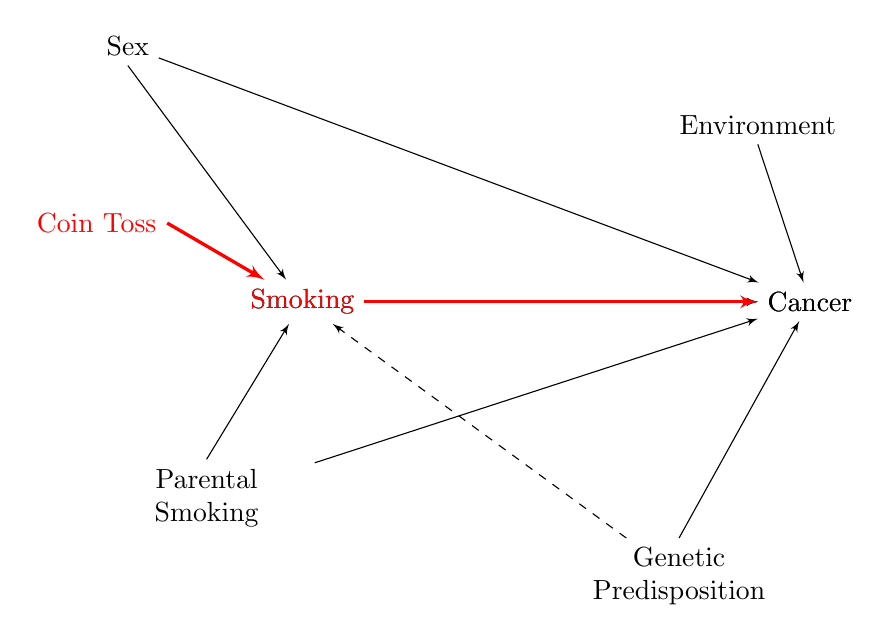
\begin{tikzpicture}[>=latex',circ/.style={draw, shape=circle, node distance=5cm, line width=1.5pt}]
    \draw<1>[->] (0,0) node[left] (X) {Smoking} -- (5,0) node[right] (Y) {Cancer};
    \draw<2>[->] (0,0) node[left, color=red] (X) {Smoking} -- (5,0) node[right] (Y) {Cancer};
    \draw[->] (-3,3) node[above] (Z) {Sex} -- (X);
    \draw[->] (Z) -- (Y);
    \draw[->] (5,2) node[above] (A) {Environment} -- (Y);
    \draw[->] (4,-3) node[below, text width=3cm, align=center] (E) {Genetic\\Predisposition} -- (Y);
    \draw[->] (-2, -2) node[below, text width=2.5cm, align=center] (W) {Parental\\Smoking} -- (X);
    \draw[->] (W) -- (Y);
    \draw[->, dashed] (E) -- (X);
    
    \draw<2->[->, very thick, color=red] (-2.5,1) node[left, color=red] (Tr) {Coin Toss} -- (X);
    \draw<2->[->, very thick, color=red] (X) -- (Y);
\end{tikzpicture}
\end{center}
\end{frame}



% design-based experimental inference
\frame{
	\frametitle{Experimental Inference I}
	\small
	\begin{itemize}\itemsep0.5em
    	\item<1-> We cannot see individual-level causal effects
    	\item<2-> We can see \textit{average causal effects}
    		\begin{itemize}
        		\item<2-> Ex.: Average difference in cancer between those who do and do not smoke
    		\end{itemize}
    	\item<3-> We want to know: $TE_i = Y_{1i} - Y_{0i}$
	\end{itemize}
}

\frame{
	\frametitle{Experimental Inference II}
	\small
	\begin{itemize}\itemsep0.5em
		\item<1-> We want to know: $TE_i = Y_{1i} - Y_{0i}$
		\item<2-> We can average: $ATE = E[Y_{1} - Y_{0}] = E[Y_{1}] - E[Y_{0}]$
		\item<3-> But we still only see one potential outcome for each unit:\\ \vspace{1em}
    		$ATE_{naive} = E[Y_{1} | X = 1] - E[Y_{0} | X = 0]$
    	\item<4-> Is this what we want to know?
	\end{itemize}
}


\frame{
	\frametitle{Experimental Inference IV}
	\small
	\begin{itemize}\itemsep0.5em
	\item What we want and what we have:
		\begin{align}
		ATE & = E[Y_{1}] - E[Y_{0}] \\[1em]
		ATE_{naive} & = E[Y_{1} | X = 1] - E[Y_{0} | X = 0]
		\end{align}		
	\item<2-> Are the following statements true?\\
  		\begin{itemize}\itemsep0.5em
      		\item<2-> $E[Y_{1}] = E[Y_{1} | X = 1]$
      		\item<2-> $E[Y_{0}] = E[Y_{0} | X = 0]$
  		\end{itemize}
  	\item<3-> Not in general!
  	\end{itemize}
}

\frame{
	\frametitle{Experimental Inference V}
	\small
	\begin{itemize}\itemsep0.5em
    	\item Only true when both of the following hold:
    	\begin{align}
    	E[Y_{1}] = E[Y_{1} | X = 1] = E[Y_{1} | X = 0]\\
    	E[Y_{0}] = E[Y_{0} | X = 1] = E[Y_{0} | X = 0]
    	\end{align}
    	\item In that case, potential outcomes are \textit{independent} of treatment assignment
		\item If true, then:
    	\begin{align*}
    	ATE_{naive} & = E[Y_{1} | X = 1] - E[Y_{0} | X = 0] \tag{5}\\
    	& = E[Y_{1}] - E[Y_{0}]\\
    	& = ATE
    	\end{align*}
	\end{itemize}
}

\frame{
	\frametitle{Experimental Inference VI}
	\small
	\begin{itemize}\itemsep0.5em
    	\item This holds in experiments because of randomization\\
    		\begin{itemize}
        		\item Units differ only in what side of coin was up
        		\item Experiments randomly reveal potential outcomes
    		\end{itemize}
    	\item<2-> Matching/regression/etc. attempts to eliminate those confounds, such that:
    	\begin{align*}
    	E[Y_{1} | Z] = E[Y_{1} | X = 1, Z] = E[Y_{1} | X = 0, Z]\\
    	E[Y_{0} | Z] = E[Y_{0} | X = 1, Z] = E[Y_{0} | X = 0, Z]
    	\end{align*}
	\end{itemize}
}


\frame{
	\frametitle{``The Perfect Doctor''}

\small
\begin{center}
\begin{tabular}{ccc}
Unit & $Y_0$ & $Y_1$ \\ \hline 
1 & ? & ? \\
2 & ? & ? \\
3 & ? & ? \\
4 & ? & ? \\
5 & ? & ? \\
6 & ? & ? \\
7 & ? & ? \\
8 & ? & ? \\ \hline
\textbf{Mean} & \textbf{?} & \textbf{?} \\
\end{tabular}
\end{center}
}

\frame{
	\frametitle{``The Perfect Doctor''}

\small
\begin{center}
\begin{tabular}{ccc}
Unit & $Y_0$ & $Y_1$ \\ \hline 
1 & ? & 14 \\
2 & 6 & ? \\
3 & 4 & ? \\
4 & 5 & ? \\
5 & 6 & ? \\
6 & 6 & ? \\
7 & ? & 10 \\
8 & ? & 9 \\ \hline
\textbf{Mean} & \textbf{5.4} & \textbf{11} \\
\end{tabular}
\end{center}
}

\frame{
	\frametitle{``The Perfect Doctor''}

\small
\begin{center}
\begin{tabular}{ccc}
Unit & $Y_0$ & $Y_1$ \\ \hline 
1 & 13 & 14 \\
2 & 6 & 0 \\
3 & 4 & 1 \\
4 & 5 & 2 \\
5 & 6 & 3 \\
6 & 6 & 1 \\
7 & 8 & 10 \\
8 & 8 & 9 \\ \hline
\textbf{Mean} & \textbf{7} & \textbf{5} \\
\end{tabular}
\end{center}
}



\frame{
\frametitle{Experimental Analysis I}
\small
\begin{itemize}
\item The statistic of interest in an experiment is the \textit{sample average treatment effect} (SATE)
\item This boils down to being a mean-difference between two groups:
	\begin{equation}
	SATE = \frac{1}{n_1}\sum Y_{1i} - \frac{1}{n_0}\sum Y_{0i}
	\end{equation}
\item In practice we often estimate this using:
	\begin{itemize}
	\item t-tests
	\item Linear regression
	\end{itemize}
\end{itemize}
}

\frame{
\frametitle{Experimental Analysis II}
	\small
\begin{itemize}\itemsep0.5em
\item We don't just care about the size of the SATE. We also want to know whether it is significantly different from zero (i.e., different from no effect/difference)
\item To know that, we need to estimate the \textit{variance} of the SATE
\item The variance is influenced by:
	\begin{itemize}
	\item Total sample size
	\item Variance of the outcome, $Y$
	\item Relative size of each treatment group
	\end{itemize}
\end{itemize}
}

\frame{
\frametitle{Experimental Analysis III}
	\small
\begin{itemize}\itemsep0.5em
\item Formula for the variance of the SATE is:\\
$\widehat{Var}(SATE) = \dfrac{\widehat{Var}(Y_0)}{N_0} + \dfrac{\widehat{Var}(Y_1)}{N_1}$

	\begin{itemize}
	\item $\widehat{Var}(Y_0)$ is control group variance
	\item $\widehat{Var}(Y_1)$ is treatment group variance
	\end{itemize}

\item We often express this as the \textit{standard error} of the estimate:\\
$\widehat{SE}_{SATE} = \sqrt{\frac{\widehat{Var}(Y_0)}{N_0} + \frac{\widehat{Var}(Y_1)}{N_1}}$
\end{itemize}
}


\frame{}

\frame{
\frametitle{Compliance}
\begin{itemize}
\item Compliance is when individuals receive and accept the treatment to which they are assigned:
	\begin{itemize}
	\item Receive the wrong treatment (cross-over)
	\item Fail to receive any treatment 
	\end{itemize}
\item This causes problems for our analysis because factors other than randomization explain why individuals receive their treatment
\end{itemize}
}

\begin{frame}
\small 
\begin{center}
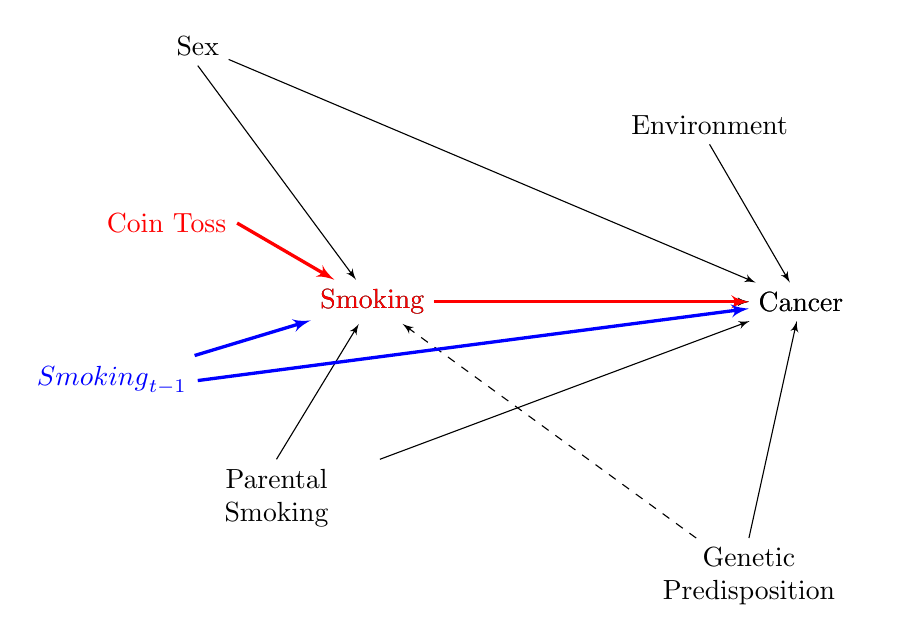
\begin{tikzpicture}[>=latex',circ/.style={draw, shape=circle, node distance=5cm, line width=1.5pt}]
    \draw<1>[->] (0,0) node[left] (X) {Smoking} -- (4,0) node[right] (Y) {Cancer};
    \draw<2->[->] (0,0) node[left, color=red] (X) {Smoking} -- (4,0) node[right] (Y) {Cancer};
    \draw[->] (-3,3) node[above] (Z) {Sex} -- (X);
    \draw[->] (Z) -- (Y);
    \draw[->] (3.5,2) node[above] (A) {Environment} -- (Y);
    \draw[->] (4,-3) node[below, text width=3cm, align=center] (E) {Genetic\\Predisposition} -- (Y);
    \draw[->] (-2, -2) node[below, text width=2.5cm, align=center] (W) {Parental\\Smoking} -- (X);
    \draw[->] (W) -- (Y);
    \draw[->, dashed] (E) -- (X);
    
    \draw[->, very thick, color=red] (-2.5,1) node[left, color=red] (Tr) {Coin Toss} -- (X);
    \draw[->, very thick, color=red] (X) -- (Y);
    \draw<2->[->, very thick, color=blue] (-3,-1) node[left, color=blue] (X2) {$\text{Smoking}_{t-1}$} -- (Y);
    \draw<2->[->, very thick, color=blue] (X2) -- (X);
\end{tikzpicture}
\end{center}
\end{frame}



\frame{
\frametitle{Ethics}
\small
\begin{itemize}\itemsep0.5em
\item Experiments raise lots of ethical considerations
\item Because we are intervening in peoples' lives, we have to weight harm and benefits of our interventions
\item A big question relates to ``deception'' (are we deceiving our experimental participants? is that a problem?)
\end{itemize}
}



\section{Quasi-Experiments}
\frame{\tableofcontents[currentsection]}

% Instruments
\frame{
	\frametitle{Why Quasi-Experiments?}
	\begin{itemize}\itemsep0.5em
		\item We are interested in the effect of $X \rightarrow Y$
		\item How can we identify the effect $X \rightarrow Y$?
		\item<2-> Relationship is confounded by unobservables
		\item<2-> We cannot manipulate $X$
	\end{itemize}
}

\frame{
	\frametitle{What is a Quasi-Experiment?}
	\small
	\begin{itemize}\itemsep0.5em
		\item Quasi-Experiments are situations where randomization-like forces influence the values of independent variables
		\item Most of the time, these are ``natural'' experiments where boundaries, discontinuities, or interruptions disrupt a continuous treatment-assignment process
		\item Analyzing a quasi-experiment involves searching for an ``instrument variable''
	\end{itemize}
}


\frame{
	\frametitle{What is ``instrumental''?}
	\begin{enumerate}\itemsep0.5em
		\item \alert<2>{serving as a crucial means, agent, or tool}
		\item of, relating to, or done with an instrument or tool
		\item relating to, composed for, or performed on a musical instrument
		\item of, relating to, or being a grammatical case or form expressing means or agency
	\end{enumerate}
}



\frame{
	\frametitle{What is ``instrumental''?}
	\begin{itemize}\itemsep1em
		\item $W$ must be a crucial cause of $X$'s effect on $Y$
		\item $W$ is the quasi-experimental shock to the causal process in our graph
			\begin{itemize}
			\item It is not caused by $X$ or $Y$
			\item It does not cause $Y$ except through $X$
			\end{itemize}
	\end{itemize}	
}

\frame{
	\frametitle{Formal Definition}
	An \textbf{instrumental variable} is a variable that satisfies two properties:\\
	\begin{enumerate}\itemsep0.5em
		\item Exogeneity\\ % Not testable
			\begin{itemize}
				\item $W$ temporally precedes $X$
				\item $Cov(B, \epsilon) = 0$
			\end{itemize}
		\item Relevance\\ % Is testable
			\begin{itemize}
				\item $W$ causes $X$
				\item $Cov(W, X) \neq 0$
			\end{itemize}
	\end{enumerate}
}



\frame{
	\frametitle{How IV Works I}
	\begin{itemize}\itemsep0.5em
		\item Start with case where $W$ is 0,1
		\item To identify the effect $X \rightarrow Y$, all we need is $W$
		\item We don't need to worry about other omitted variables, but we don't learn anything about the rest of the causal graph
	\end{itemize}
}

\begin{frame}
\small 
\begin{center}
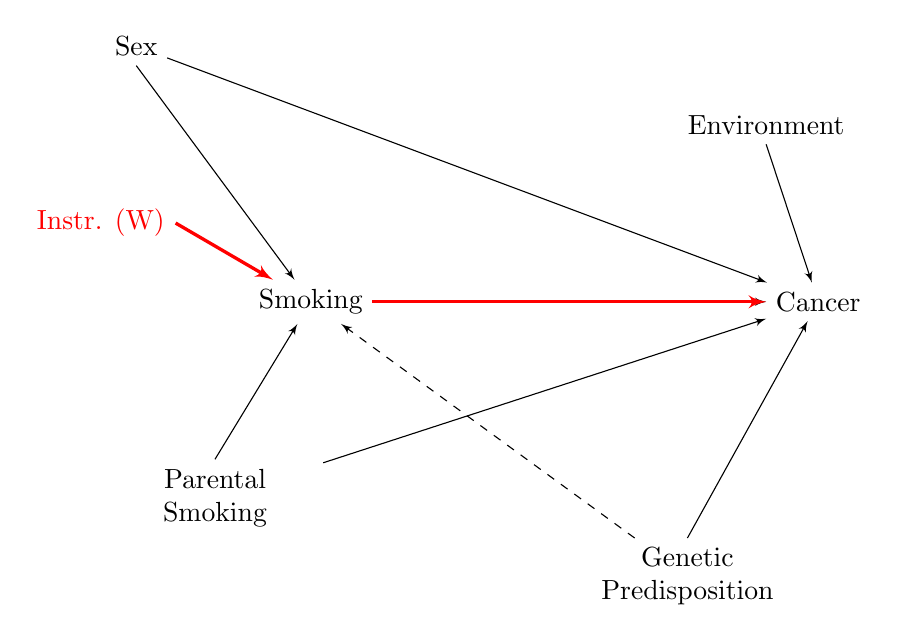
\begin{tikzpicture}[>=latex',circ/.style={draw, shape=circle, node distance=5cm, line width=1.5pt}]
    \draw[->] (0,0) node[left] (X) {Smoking} -- (5,0) node[right] (Y) {Cancer};
    \draw[->] (-3,3) node[above] (Z) {Sex} -- (X);
    \draw[->] (Z) -- (Y);
    \draw[->] (5,2) node[above] (A) {Environment} -- (Y);
    \draw[->] (4,-3) node[below, text width=3cm, align=center] (E) {Genetic\\Predisposition} -- (Y);
    \draw[->] (-2, -2) node[below, text width=2.5cm, align=center] (W) {Parental\\Smoking} -- (X);
    \draw[->] (W) -- (Y);
    \draw[->, dashed] (E) -- (X);
    
    \draw[->, very thick, color=red] (-2.5,1) node[left, color=red] (Tr) {Instr. (W)} -- (X);
    \draw[->, very thick, color=red] (X) -- (Y);
\end{tikzpicture}
\end{center}
\end{frame}

\frame{
	\frametitle{How IV Works II (Wald)}
	\small
	\begin{itemize}\itemsep0.5em
		\item Imagine two effects:
		\begin{align}
		ITT_Y & = E[Y | W = 1] - E[Y | W = 0]\\
		ITT_X & = E[X | W = 1] - E[X | W = 0]
		\end{align}
		\item IV estimates the LATE: $\dfrac{ITT_X}{ITT_X}$
		\item In a regression, this is:\\
			$E[Y|W] = \beta_0 + \text{LATE} \times E[X|W]$
	\end{itemize}
}


\frame{
	\frametitle{{\large Local Average Treatment Effect}}
	\small
	\begin{itemize}\itemsep0.5em
	\item IV estimate \textit{local} to the variation in $X$ that is due to variation $W$ (i.e., the LATE)
	\item This matters if effects are \textit{heterogeneous}
	\item LATE is effect for those who \textit{comply} with instrument
	\item Four subpopulations:
		\begin{itemize}\small
		\item Compliers: $X = 1$ only if $W = 1$
		\item Always-takers: $X = 1$ regardless of $W$
		\item Never-takers: $X = 0$ regardless of $W$
		\item Defiers: $X = 1$ only if $W = 0$
		\end{itemize}
	\end{itemize}
}




\frame{
	\frametitle{Finding Instruments}
	\begin{itemize}\itemsep0.5em
		\item Forward, not backward, causal inference
		\item Most instruments are not things we care about
			\begin{itemize}
				\item Weather, disasters
				\item Geography, borders, climate
				\item Lotteries
			\end{itemize}
		\item A good instrument is one that satisfies both of our conditions, so we need:
			\begin{itemize}
				\item A good story about exogeneity
				\item Evidence that instrument is \textit{strong}
			\end{itemize}
	\end{itemize}
}



\frame{
	\frametitle{Conclusion}
	\small
	\begin{itemize}
	\item In \textbf{regression}/\textbf{matching}, we address confounding through conditioning on observable variables
	\item In \textbf{quasi-experiments}, we address confounding and ordering through experiment-like discontinuities or interventions that occur at specific points in time for specific subsets of units
	\item In \textbf{experimentation}, we solve confounding and ordering through \textit{randomized} intervention
	\end{itemize}
}

\frame{}

\frame{
	\frametitle{Preview}
	\begin{itemize}
	\item Next week: The End!!
	\end{itemize}
}

\appendix
\frame{}

\end{document}
